\documentclass[border=1pt]{standalone}
\usepackage{tikz}
\usetikzlibrary{arrows.meta}
\usepackage{mathptmx}
\begin{document}
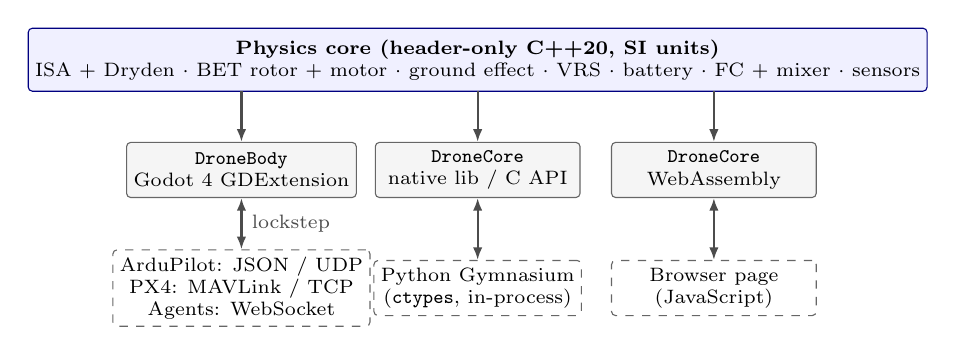
\begin{tikzpicture}[font=\scriptsize,
  box/.style={draw=black!60, rounded corners=1.5pt, align=center, inner sep=2.5pt,
              minimum height=7mm, minimum width=26mm, fill=black!4},
  ext/.style={box, dashed, fill=white},
  arr/.style={-{Latex[length=1.6mm]}, black!70, thick},
  barr/.style={{Latex[length=1.6mm]}-{Latex[length=1.6mm]}, black!70, thick}]
\node[draw=blue!50!black, fill=blue!6, rounded corners=1.5pt, align=center,
      minimum width=86mm, minimum height=8mm, inner sep=2.5pt] (core) at (0,0)
  {\textbf{Physics core (header-only C++20, SI units)}\\
   ISA + Dryden $\cdot$ BET rotor + motor $\cdot$ ground effect $\cdot$ VRS $\cdot$
   battery $\cdot$ FC + mixer $\cdot$ sensors};
\node[box] (godot) at (-30mm,-14mm) {\texttt{DroneBody}\\Godot 4 GDExtension};
\node[box] (lib)   at (0,-14mm)     {\texttt{DroneCore}\\native lib / C API};
\node[box] (wasm)  at (30mm,-14mm)  {\texttt{DroneCore}\\WebAssembly};
\node[ext] (fw)    at (-30mm,-29mm) {ArduPilot: JSON / UDP\\PX4: MAVLink / TCP\\Agents: WebSocket};
\node[ext] (py)    at (0,-29mm)     {Python Gymnasium\\(\texttt{ctypes}, in-process)};
\node[ext] (br)    at (30mm,-29mm)  {Browser page\\(JavaScript)};
\foreach \n/\x in {godot/-30mm, lib/0mm, wasm/30mm}
  \draw[arr] (\x,-4mm) -- (\n.north);
\draw[barr] (godot.south) -- node[right]{lockstep} (fw.north);
\draw[barr] (lib.south) -- (py.north);
\draw[barr] (wasm.south) -- (br.north);
\end{tikzpicture}
\end{document}
